%File: mume_paper.tex
\documentclass[letterpaper]{article}
\usepackage{mume}
\usepackage{times}
\usepackage{helvet}
\usepackage{courier}
\usepackage{url}
\usepackage{booktabs}
\usepackage{graphicx}
\frenchspacing
\setlength{\pdfpagewidth}{8.5in}
\setlength{\pdfpageheight}{11in}

\hyphenation{Muse-Score}

\pdfinfo{
/Title (Comparative Analysis of Key Inference Methods from Monophonic Melodies in Symbolic Pop Music)
/Author (Anonymized)}
%/Author (Paul M. Bodily, Dan Ventura)}
\setcounter{secnumdepth}{0}  
\begin{document}
	% The file mume.sty is the style file for MUME 
	% proceedings, working notes, and technical reports.
	%
\title{Comparative Analysis of Key Inference Models for Musical Metacreation}
\author{Paul M. Bodily and Dan Ventura\\
Department of Computer Science\\
Brigham Young University\\
Provo, UT 84602-6576\\
}
	\maketitle
	\begin{abstract}
		\begin{quote}
%Background
Creative musical systems must be equipped with certain intelligent abilities to understand fundamental aspects of music, particularly in order to autonomously interact with other creative agents. Key inference, a relatively simple task for trained human experts, is one such intelligent ability required to normalize and analyze melodic compositions. We assess the accuracy of several traditional and machine learning approaches to the key and key signature inference problems on a dataset of 480 melodies in MIDI format. We compare these accuracies with those of trained human musicians on the same tasks. We evaluate the impact of including note duration and note repetition as learning features. We find machine learning approaches outperform traditional key inference methods. The highest accuracies (0.729 for key inference and 0.896 for key signature inference) were achieved using a 4-gram language model. Including note duration improved the results of traditional approaches when inferring key, but had the opposite effect for key signature inference. Our findings suggest that the key of a melodic passage depends more heavily on the sequence of the notes rather than their frequency or distribution.
		\end{quote}
	\end{abstract}
	
\section{Introduction}

A fundamental element of musical metacreation is the quest to ``[endow] machines with creative behavior'' \cite{pasquier2012preface}. Such behavior in humans draws on a full spectrum of intelligent abilities \cite{colton2012computational}. Often there are overlaps in the intelligent abilities that are required for different tasks. This has been noted to be especially true of musical computational creative systems \cite{bodily2017hbpl}.

An example of such an ability is \emph{musical key inference}: the ability to recognize the group of pitches or scale that form the basis of a particular composition. This ability is a relatively simple task for trained human musicians. The key or tonic of a passage is used to transpose passages, motifs, and progressions to a common tonal center in order to be able to compare relationships and functions of pitched elements across musical selections in different keys.

In computational systems data often comes pre-labeled with the key. However, humans and music systems alike are often placed in unsupervised training scenarios in which the key is not labeled, but must rather be inferred. This inference is critical, particularly for interactive agents which must interpret and respond to other music agents. The key in which systems improvise or compose is often not explicitly communicated by other performing agents but is rather inferred from what \emph{is} explicitly communicated (i.e., notes, chords, etc.). In the quest for creating autonomous, interactive musical agents, to what extent can this skill of inferring musical key be learned?

The \emph{key} or tonality is a root pitch or \emph{tonic} and modality (e.g., major, minor, etc.) which forms the structural basis for Western art music from Baroque to Romantic, along with much modern popular music. This tonality provides a context within which ``the melodic and harmonic unfolding of a composition takes place'' \cite{vos1996parallel}. Even the untrained ear appreciates the structure, tension, and resolution that tonality provides. Each key is associated with a \emph{key signature} representing the specific pitches that belong to the scale represented by the key. There exists a many-to-one relationship between keys and key signatures. For example, each major key and its \emph{relative natural minor key} (whose root is three half steps lower) are associated with the same key signature. Though music certainly exists with keys whose modes are not strictly major or minor, we have as a simplifying assumption chosen to focus solely on these two common modes. Note that we are not interested in inferring harmonic accompaniment (cf. \cite{groves2013automatic}), but rather in determining the main key and key signature of a piece of music.

Our interest in this problem arises as both a matter of necessity and as a philosophical inquiry. In efforts to apply machine learning to the generation of pop lead sheets, much of the freely available training data in the pop genre exists in MIDI format. Unlike more amenable formats (e.g., Music XML), MIDI files do not typically contain information about key or key signature. In order to train machine learning models on this data, inferring key and/or key signature is useful for being able to ``normalize'' pitches into a common key. Also for viewing MIDIs with music notation software (e.g., MuseScore), key signature is an important notational element.

Besides these practical applications, the question is of broader philosophical interest: how is it that a human musician can listen to a musical selection and infer its key? There is a profound irony in the contrast between knowing how and being able to explain how to infer the key of a musical selection. Expert musicians routinely and accurately perform this task. However the description for their methodology is often inexact and derives from finding the key that ``feels'' right, provides a sense of ``finish'', or the key where the music ``lands''. One common supposition is that the solution involves finding the key which minimizes the total number of accidentals in a composition \cite{gorow2011hearing}. Part of our purpose is to test this hypothesis by comparing this approach with several machine learning algorithms. Examining algorithms that perform well on this task may help provide some insight into how human musicians infer key.

We hypothesize that a monophonic melodic sequence alone is sufficient in many cases to determine key. We have chosen to focus on monophonic melodies, again, for both practical and philosophical reasons. First, though compositions have varying amounts of harmonic context, the monophonic melody acts as a common denominator in all compositions in our dataset. Second, humans---in singing, humming, whistling, or playing a monophonic instrument---are able to communicate and interpret music based on monophonic melody. Picture, for example, singing a melody to a musical friend that had never heard it. Without specifying either the key or tonic, the friend is able to infer this information with some probability in order to make sense of what (s)he is hearing (e.g., melody starts on the major third, ends with the tonic, etc.). Thus the ability to infer tonality for monophonic melodies represents an AI task if computers are to effectively understand and communicate with humans.

We test our hypothesis on a dataset of 480 pop melodies in MIDI format\footnote{Metadata are available at \url{http://popstar.cs.byu.edu/metadata_for_midis.csv}}. Data were selected to exclude melodies with modulation or key changes. As a fundamental building block of music knowledge and creativity, effective key inference models stand to add increase autonomy in musical metacreation systems.

\section{Related Work}

Several previous studies have examined key inference in various contexts, though to our knowledge ours is the first attempt to do so using \emph{n}-gram models with monophonic pop melodies.

Krumhansl matches the relative frequencies and durations with which tones are sounded (which she terms a \emph{tonal hierarchy}) of a composition against the known tonal hierarchies of each key (\citeyear{krumhansl2001cognitive}). This algorithm was applied to infer keys for compositions from three classical composers: Bach, Chopin, and Shostakovich. 

The key-finding algorithm of Longuet-Higgins and Steedman successively eliminates keys based on the presence or absence of the notes of the composition in each of the major and minor scales \cite{longuet1971interpreting}. Holtzman (\citeyear{holtzman1977program}) infers key from the prevalence of common key-defining intervals (e.g., triads, tonic-fifths, tonic-thirds). Both algorithms were applied to Bach's \emph{Well-Tempered Clavier}.

Hu and Saul use Latent Dirichlet Allocation (LDA)---a statistical approach for discovering hidden topics in large corpora of text---for key-finding, looking for common co-occurrences of notes in music. Their model essentially treats keys like topics. They then model compositions as a random mixture of key-profiles, allowing them to track modulations (\citeyear{hu2009probabilistic}). Temperley interprets the traditional key-profile model (proposed by \citeauthor{krumhansl2001cognitive} (\citeyear{krumhansl2001cognitive}) and subsequently modified by \citeauthor{temperley1999s} (\citeyear{temperley1999s})) as a Bayesian probabilistic model and discusses the implications of the connection between these two models (\citeyear{temperley2002bayesian}). All applications of the model are on the Kostka-Payne corpus, a collection of textbook excerpts of tonal music. Vos and Van Geenen present a parallel search key-finding algorithm for single-voiced music. Notes are evaluated against both the scalar and the chordal structures of each key. They demonstrate the model's effectiveness on Bach's \emph{Well-Tempered Clavier} (\citeyear{vos1996parallel}). Zhu et al. present a method for key estimation in audio pop and classical music (\citeyear{zhu2005music}). Their method performs marginally higher with pop music than with classical music. 

Much recent work has been devoted to inferring key from audio music. Shenoy et al. outline a rule-based algorithm for finding key from audio musical signals using chroma based frequency analysis and chord progression patterns (\citeyear{shenoy2004key}). Mauch and Dixon infer chords and key simultaneously from audio (\citeyear{mauch2010simultaneous}). Chafe et al. extract symbolic music from audio from which meter and key are inferred (in that order) (\citeyear{chafe1982toward}). The key-recognizer assumes that rhythmic and melodic accent points are significant features for inferring key.

\citeauthor{temperley2013statistical} (\citeyear{temperley2013statistical}) address key-finding in rock songs from harmonic, melodic, and combined harmonic-melodic data. They compare a key-profile method (a normative distribution of scale-degrees) and a key-profile method weighted by note durations for key-finding in monophonic rock melodies. Their findings suggested that the weighted method worked somewhat better. Their work provides an excellent survey of the work done on key-finding algorithms in both pop and classical music, both from audio and sheet music.

\section{Methods}

\subsection{Data}

We collected 480 melodies from 278 pop artists representing music spanning several decades (see Figure~\ref{tab:data_summary}). Songs were compiled from several online MIDI databases and keys (inferred from melody together with harmonic context) were manually labeled by trained musicians. We were pleased to find that every key was represented by at least two songs (see Figure~\ref{fig:key_distribution}). Only songs with a single key were selected for our experiments (no modulations). Melody notes were isolated from the MIDI files. The melody for the entire song was used for inference purposes.

\begin{figure}
  \centering
 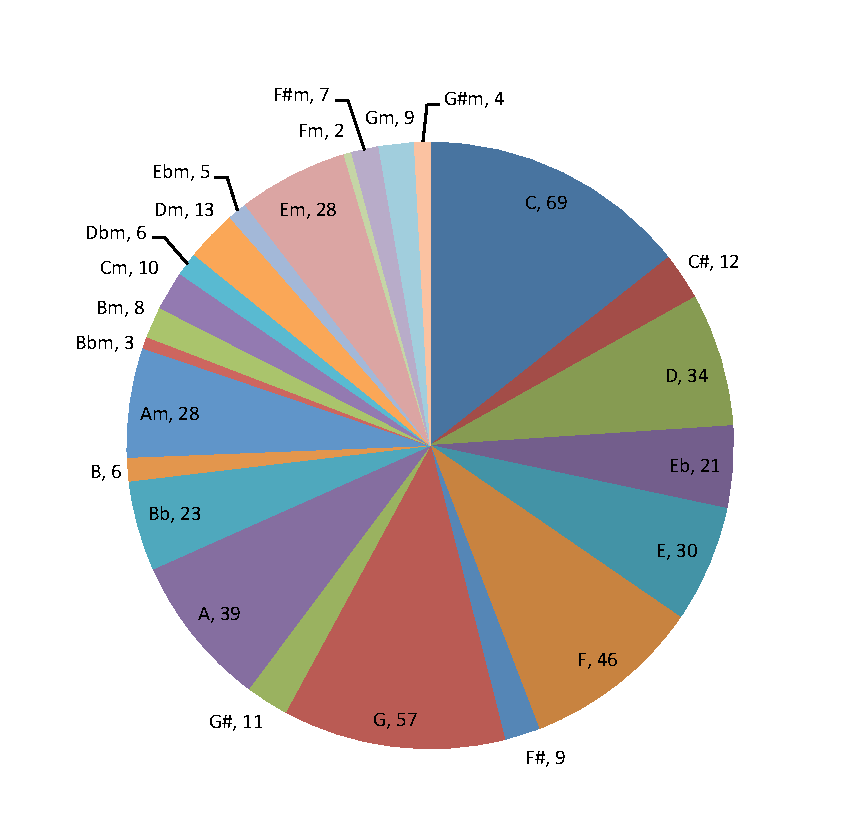
\includegraphics[width=.4\textwidth]{./key_distribution.pdf}
  \caption{\emph{Key distribution of pop melodies}. Every key is represented at least twice in the subset of melodies. In general keys with fewer sharps and flats are more highly represented.}
  \label{fig:key_distribution}
\end{figure}

\begin{table}[]
\centering
\caption{Highly Represented Pop Artists}
\label{tab:data_summary}
\begin{tabular}{@{}lc@{}}
\toprule
Artist & \# of songs\\ \midrule
Beatles	& 28 \\
Elvis Presley	& 13 \\
Kiss	&	11 \\
Madonna	&	8 \\
Eagles	&	6 \\
Aerosmith	&	6 \\
Elton John	&	6 \\
U2	&	6 \\
Beach Boys	&	5 \\
Michael Jackson	&	5 \\
Pink Floyd	&	5 \\
Bobby Vee		&	5 \\
Adele	&	5 \\
Queen	&	4 \\
Kinks		&	4 \\
\end{tabular}
\end{table}

\subsection{Implementation}

We compared the accuracy of 4 traditional and 5 machine learning methods against the accuracy of trained musicians (different than those employed for labeling ground truth) on the tasks of inferring key and key signature for pop melodies\footnote{source available at \url{http://popstar.cs.byu.edu/find_key.py}}. For each key signature there is a major and minor key and thus key inference---which precludes key signature inference---represents the more difficult of the two tasks. For the machine learning methods, we used 10-fold cross validation for training and testing.

\emph{Minimize Accidentals by Count}. This algorithm represents the common theory that the best key is that which minimizes the number of resulting accidentals.

\emph{Minimize Accidentals by Duration}. Similar to the previous method but finds the key which minimizes the total duration of accidentals.

\emph{Root Mean Squared Error (RMSE) of Pitch Count Profiles}. Similar to the method followed by \citeauthor{krumhansl2001cognitive} (\citeyear{krumhansl2001cognitive}) and others, we generated pitch profiles. Rather than generate profiles for each major and minor key, we chose to generate a single profile for all major keys and a second for all minor keys. This decision is based on the assumption that the variation in pitch distribution varies very little (if at all) as compared to the distributional variation between the major and minor modes. Major and minor mode pitch profiles were generated from the pitch counts in training instances transposed to either the C major or A minor keys depending on whether the instance was major or minor. A pitch profile is created for each test instance, transposed into each of the 12 possible keys. Each transposed profile is compared to both the major and minor generic pitch profiles using RMSE. The transposed pitch profile and the major/minor pitch profile with the minimum RMSE value are used to infer key and modality.

\emph{RMSE of Pitch Duration Profiles}. Similar to the previous method but pitch profiles are generated from pitch durations rather than mere counts (see Figure~\ref{fig:pitch_profiles}). 

n\emph{-gram Models}. An n-gram model calculates the probability of the next token given some context window of length \emph{n} \cite{brown1992class}. These probabilities are learned from the sequence of notes in the training instances and then used to calculate the probability of note sequences in the test instances. We trained \emph{n}-gram models for values of \emph{n} from 1 to 5, using Laplace smoothing and a pseudocount alpha value of 1. For each value of \emph{n} a single \emph{n}-gram model was trained for melodies in major keys and another for melodies in minor keys. Probabilities were normalized across both models. Test instances were than transposed and scored by each trained model. The transposition and model which maximized the probability of the test instance determined the key and modality.

In addition to the methods described above, we also report accuracy from four other sources. First, the \emph{baseline} accuracy represents the approach of always guessing the most common class. \emph{MIDI Annotations} refers to the key signature that was originally given in the MIDI file (if any was provided). We report the accuracy of a third-party MIDI-reader called \emph{MuseScore}. Insofar as MIDI is not a symbolic music format, many files fail to include (accurate) information about key or time signature, thus motivating the need to infer this information from the notes themselves. This functionality is built in with varying success to many programs which render MIDI files as sheet music. MuseScore (version 2.0.3) is one such program. Despite not having access to the MuseScore algorithm, we manually opened and examined each song from the database in MuseScore to record the result of their key inference algorithm. We include the accuracy of MuseScore's inferred key-signature in our results for comparison.

Lastly, we enlisted 15 trained musicians to complete the same melodic key inference task. Each musician was afforded access to a keyboard and asked to listen to 20 melodies (the first of which was a control melody, \emph{God Rest Ye Merry Gentlemen}---all respondents answered the control key correctly) without access to printed scores. In addition to labeling the key and key signature for each melody, respondents were asked to indicate how familiar they were with the melody\footnote{Survey results and self-reported musician training information are available at \url{http://popstar.cs.byu.edu/raw_survey_results_name_key.csv}}. This was to control for bias that might arise as a result of prior knowledge of the harmonic context of the melody. We report the accuracies on the melodic key inference task as a function of the degree of familiarity as well as an overall weighted average of these three scores.

\begin{figure}
  \centering
 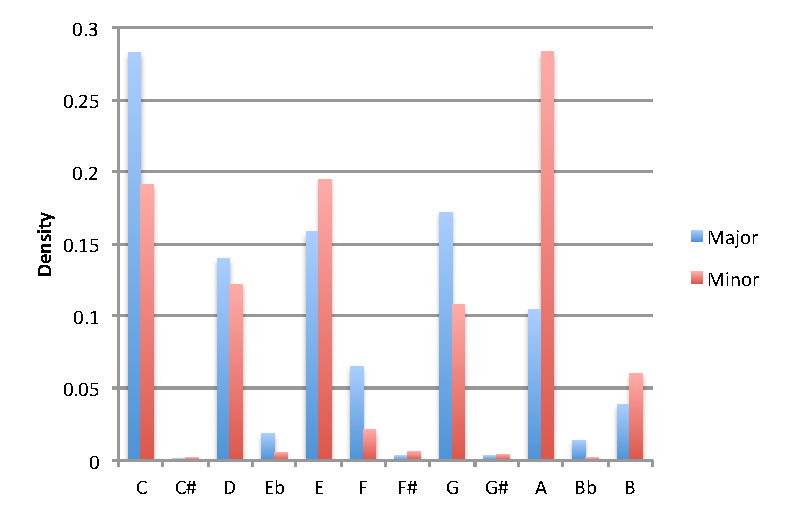
\includegraphics[width=.5\textwidth]{./PitchProfilesWeighted.pdf}
  \caption{\emph{Weighted Major/Minor Pitch Profiles}. Profiles are based on the duration of pitches in each of the major and minor modes. Profiles for major keys (blue) have been normalized to C major and those for minor keys (red) to A minor. Note that the A pitch is relatively more frequent for minor keys (where it functions as the tonic) than for major keys (where it functions as the 6th from the root). Likewise the G pitch is relatively more frequent for major keys (where it functions as the dominant) than for minor keys (where it functions as the 7th from the root).}
  \label{fig:pitch_profiles}
\end{figure}

\section{Results}

Results are shown in Table~\ref{tab:results}. We report accuracy both for inferring the key and for inferring the key signature. Inasmuch as key signature is a more generic classification of key (e.g., C major and A minor both have a key signature with no flats or sharps), accuracy for key signature will always be better than accuracy for key.
\begin{table}[]
\centering
\caption{Key Finding Accuracy for Pop Melodies}
\label{tab:results}
\begin{tabular}{@{}lll@{}}
\toprule
Method & Key & Key Signature \\ \midrule
Baseline (C)	&	0.144 	&	0.202 \\
MIDI	Annotations		&	n/a		&	0.483 \\
MuseScore	&	n/a		&	0.746 \\ \midrule
Minimize Accidentals	 by Count	&	0.494 &		0.660 \\
Minimize Accidentals	 by Duration	&	0.490 &		0.665 \\
RMSE of Pitch Count Profiles	&	0.606	&	0.796	\\
RMSE of Pitch Duration Profiles	&	0.613	&	0.765	\\ \midrule
Unigram model    	&	0.629	& 0.815       \\
Bigram model		&	0.654	&	0.883	\\
Trigram model		&	0.679	&	0.883	\\
4-gram model		&	\emph{0.729} &	\emph{0.896}	\\
5-gram model		&	0.700 &	0.885              \\ \bottomrule
Human (``I know this song'')		&	0.846	&	0.865	\\
Human (``Sounds familiar'') 		&	0.75 &	0.786	\\
Human (``I don't know this song'')		&	0.676 &	0.815              \\ \midrule
Human Average		&	0.719 &	0.822              \\\bottomrule
\end{tabular}
\end{table}

\section{Discussion}

Normalizing to a common key really only requires that we identify the key signature for a composition without regard for whether the key is the major key associated with the key signature or its relative minor. We chose to model the major and minor separately based on the hypothesis that the melodies that each produces would be sufficiently different to warrant creating individual profiles.The key inference methods which minimize the frequency of accidentals show the most dramatic improvement because these methods inherently fail to provide a way of distinguishing between a major key and its relative minor.

We encountered several challenges, primarily centered around assumptions made about the modalities present in our dataset. Songs based on blues scales often include a flat seven (which would suggest a key a fifth below the actual tonic) or both the major and minor third. Hard rock songs often exclude the third all-together, making it difficult to infer whether a major or minor key signature is more accurate. This finding supports the argument made by \citeauthor{temperley2013statistical} (\citeyear{temperley2013statistical}) and others against the applicability of the major/minor dichotomy to rock music. These confounding influences are reflected in the confusion matrices for classifications of songs in these genres (see Figure~\ref{fig:confusion_matrix}).

\begin{figure*}[h]
  \centering
 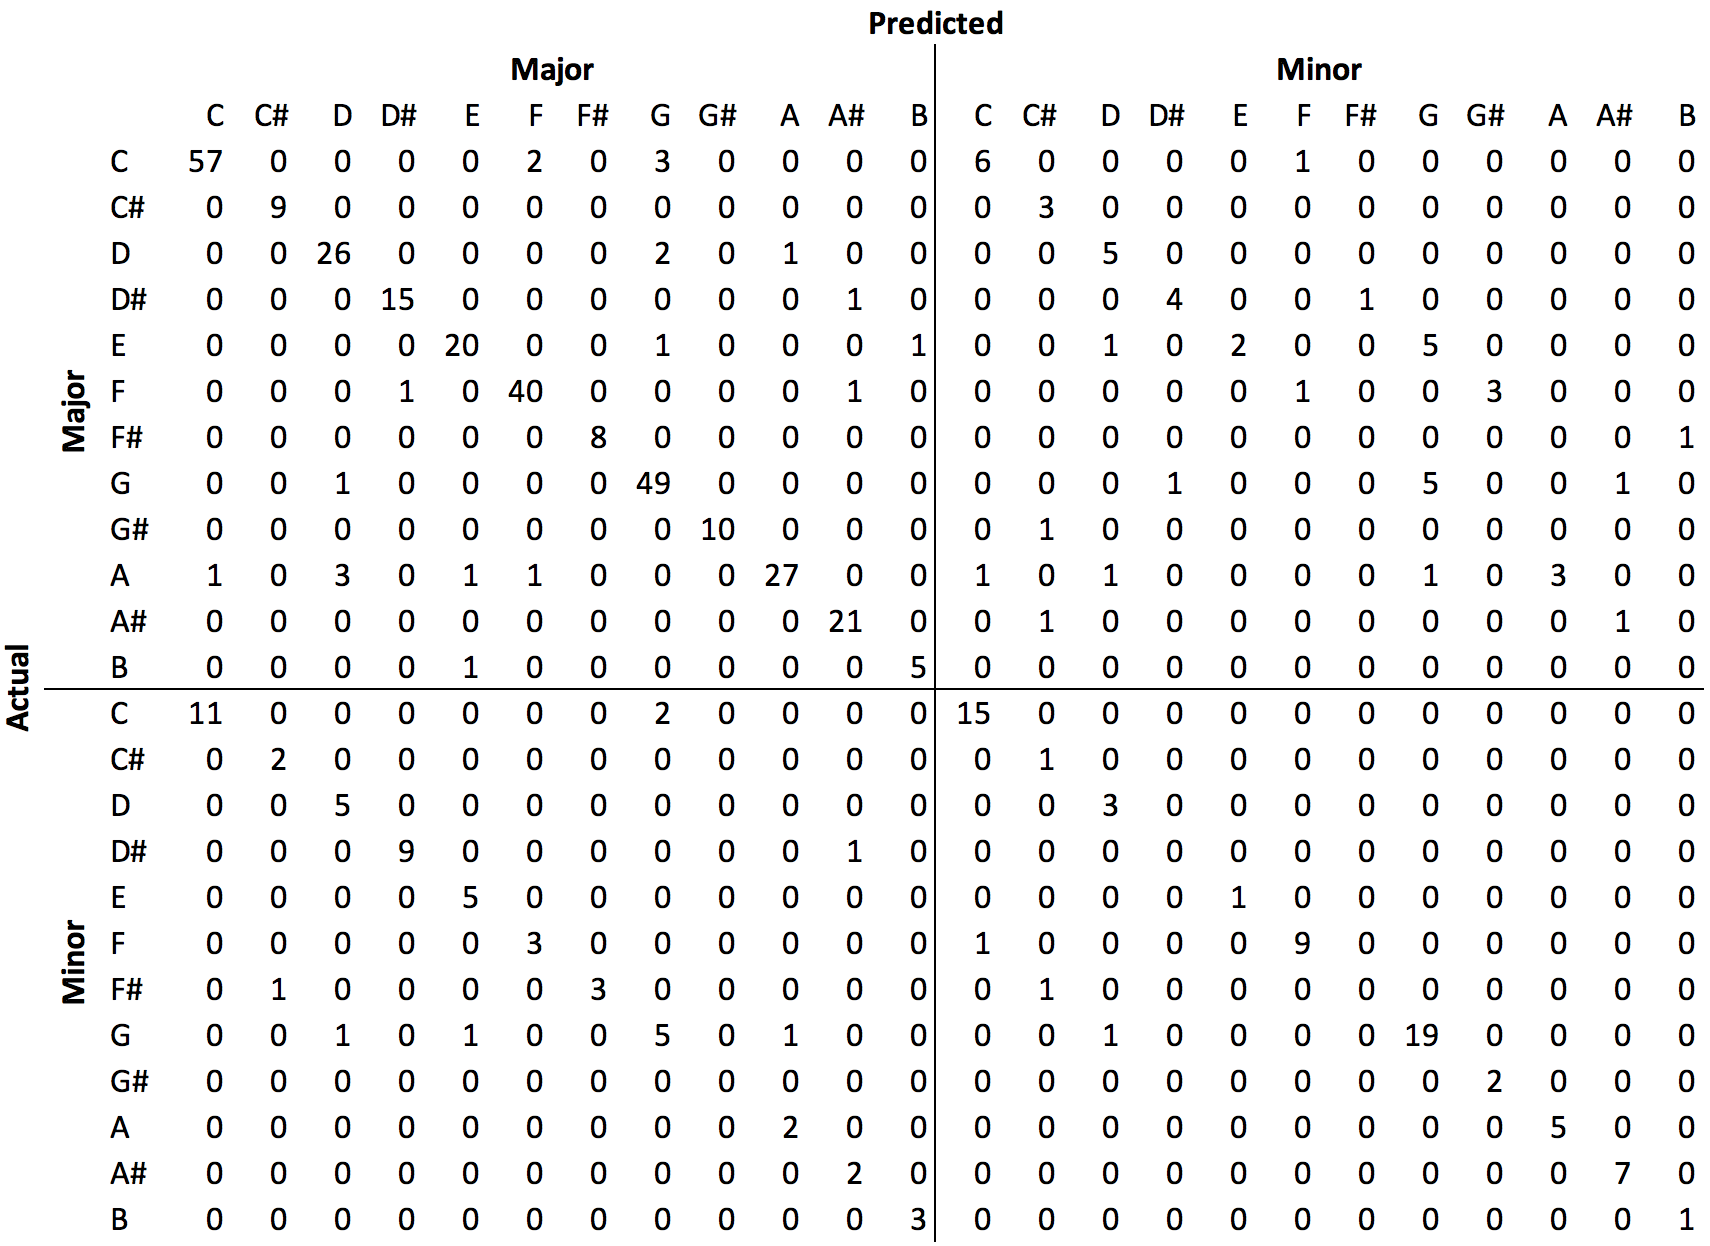
\includegraphics[width=\linewidth]{./confusion_matrix.png}
  \caption{\label{fig:confusion_matrix}\emph{Key Inference Confusion Matrix for 4-gram model}. Much of the mis-classification confuses major and minor modes for the same key. In cases such as hard rock which use open fifths and exclude the third completely the mode (i.e., major or minor) is difficult to establish.}
\end{figure*}

As regards the \emph{n}-gram models, we note that the unigram model is essentially equivalent to a pitch profile rendered as an applied probability distribution, and thus it seems reasonable that it should perform about on par with the RMSE of Pitch Count Profile method.

We increased the value of \emph{n} until we observed a decrease in accuracy. As is typical of \emph{n}-gram models, as \emph{n} increases, the model begins to essentially memorize the training data at which point the differences between test and training sets become as significant as the differences between the inferred key classes.

It is important to note that although our best accuracy on key-finding (.729) is significantly below the values reported by studies mentioned in the related works, the task of inferring key from melody is significantly more challenging than inferring key from songs which include harmony. This is evidenced by the relative accuracies of the algorithmic and human performances on the melodic key inference problem. 

It should also be considered that human listeners that are familiar with a melody may more accurately infer key from having familiarity with the harmony also. This is evidenced in our results in the fact that the more familiar the human listeners were with the song being played, the higher the accuracy on the key inference problem. Notably the same was not necessarily true with the key signature inference, suggesting that without knowledge of the context, humans may confuse a major and relative minor for an unknown melody but still infer the correct key signature. This is also evidenced by the confusion matrix for the 4-gram model, shown in Figure~\ref{fig:confusion_matrix}. We therefore express confidence in the reported accuracies of these models.

It is of interest to note that the \emph{n}-gram models generally outperformed the human models on the key signature inference task. The 4- and 5-gram models outperformed the human respondents on the key inference task when the human was otherwise unfamiliar with the song being played. 

Our results suggest that considering pitch counts or durations is less effective than a model which considers the sequence of pitches. This agrees with our intuition insofar as many pop songs spend the bulk of their duration progressing through chords which are not the root and may not even be closely related to the root. Notions of resolution and finding where the song ``lands'' inherently suggest that the contour and progression of the notes matters more than their frequency. The key is often most clearly defined at the beginning and ends of musical phrases or the beginning and end of the song itself. Whereas the method of counting note frequencies fails to give higher weight to these defining regions of the melodic passage, this information is embedded within the probabilistic framework of \emph{n}-gram models which employ a special n-gram for the beginning and end of sequences.

We find the superior accuracy of \emph{n}-gram models to the MuseScore key-signature inference model to be particularly promising inasmuch as it suggests that an \emph{n}-gram model might be used to improve the state of the art in industrial MIDI-reading software.

As regards key inference from monophonic pop melodies, we find that machine learning methods (\emph{n}-gram language models in particular) perform better than traditional key-finding algorithms, though both improve upon baseline accuracy. We also envision developing a framework for detecting key \emph{modulations} in pop melodies and using normalized unlabeled melodic data for compositional analysis. 

\section{Conclusion}

We have examined several solutions to the task of inferring key and key signature in monophonic music sequences. We found that for the particular case of monophonic sequences, the 4-gram model performed best at both identifying key and key signature. Endowing musical creative systems with intelligent abilities like key inference increases their autonomy. As key is a fundamental concept to many genres of music, this computational subconcept model can be modularly reused to improve musical metacreation across several domains.

\bibliographystyle{mume}
\bibliography{bibfile1}
\end{document}
